\section{Ergonomische Inspektion}

Eine der relevanten Aufgaben, die zu Beginn der Analyse einer Schnittstelle durchgeführt werden muss, ist eine ergonomische Inspektion der Schnittstelle.
Diese Aufgabe erfordert nur das Wissen, das für diese Bewertung erforderlich ist, keine Drittparteien oder externen Benutzer.

Für diese Inspektion werde ich mich hauptsächlich auf die ergonomischen Kriterien stützen, die von J. M. C. Bastien und D. L. Scapin in ihrem Artikel \textit{Ergonomic Criteria for the Evaluation of Human-Computer Interfaces}\cite{bastienscapin}.
Diese Kriterien, die in acht Punkte unterteilt sind, wurden entwickelt, um die Dimensionen der Funktionalität einer Schnittstelle zu definieren und zu operationalisieren.

Sie können folgendermaßen zusammengefasst werden:

\begin{table}[H]
  \begin{tabular}{p{0.25\linewidth} |p{0.5\linewidth}|p{0.25\linewidth}}
    Name                  & Beschreibung                                                                                                                                                                                 & Unterkriterien                                                            \\ \hline\hline

    Guidance              & Mittel, die zur Verfügung stehen, um die Benutzer während ihrer Interaktion mit einem Computer zu beraten, zu orientieren, zu informieren, anzuweisen und zu leiten                          & Prompting, Grouping/Distinction of Items, Immediate Feedback, Legibility. \\\hline
    Workload              & betrifft alle Schnittstellenelemente, die eine Rolle bei der Verringerung der wahrnehmungsbedingten oder kognitiven Belastung der Nutzer und bei der Steigerung der Dialogeffizienz spielen. & Brevity, Information Density                                              \\\hline
    Explicit Control      & Verarbeitung expliziter Benutzeraktionen durch das System und die Kontrolle, die die Benutzer über die Verarbeitung ihrer Aktionen durch das System ausüben.                                 & Explicit User Action,  User Control                                       \\\hline
    Adaptability          & Fähigkeit, sich kontextabhängig und entsprechend den Bedürfnissen und Vorlieben der Nutzer zu verhalten                                                                                      & Flexibility, User Experience                                              \\\hline
    Error Management      & Vorbeugung und Reduzierung von Fehlern und Behebung von Fehlern, wenn sie auftreten                                                                                                          & Error Protection, Quality of Error Messages, Error Correction             \\\hline
    Consistency           & die Art und Weise, in der Entscheidungen für das Schnittstellendesign in ähnlichen Kontexten beibehalten werden und in unterschiedlichen Kontexten anders ausfallen                          &                                                                           \\\hline
    Significance of Codes & Beziehung zwischen einem Begriff und/oder einem Zeichen und seiner Referenz.                                                                                                                 &                                                                           \\\hline
    Compatibility         & Übereinstimmung zwischen den Merkmalen der Benutzer und den Merkmalen der Aufgabe sowie die Organisation der Ausgaben, Eingaben und des Dialogs für eine bestimmte Anwendung,                &
  \end{tabular}
  \caption{Zusammenfassung der ergonomischen Kriterien von Bastien und Scapin}
\end{table}

Die Inspektion wurde über einen Zeitraum von zwei Wochen durchgeführt. Die Methodik bestand darin, für jedes Kriterium alle Seiten der Benutzeroberfläche durchzugehen und Mängel zu identifizieren.
Dies führte zu einem Inspektionsbericht (pdf-Version in Englisch \ref{dryad-ergonomic-inspection}), in dem jedes Problem detailliert und mit einem Lösungsansatz beschrieben wurde. Angesichts der umfassenden Liste mussten die Aufgaben priorisiert werden.
Dies geschah in Absprache mit dem Cloud-Team.
Die kritischsten Punkte werden in den folgenden Abschnitten nach Kriterien gegliedert.

\subsection{Guidance} \label{sec:guidance}

Ein häufig anzutreffender Mangel in Schnittstellen ist das Fehlen von Labels in den Eingaben eines Formulars oder das Verwenden nur eines Icons.
Dies passt zum Unterkriterium \textit{Prompting} und stellt ein echtes Verständnisrisiko für den Nutzer dar.
Obwohl viele Icons von der Mehrheit der Menschen als üblich angesehen werden, bleibt es ein Risiko, sie zu verwenden, vor allem, wenn die Schnittstelle für mehrere Kulturtypen oder mehrere Ebenen der Computerkenntnisse auf Seiten der Benutzer bestimmt ist.
P. Pappachan und M. Ziefle haben in ihrer Studie \textit{Cultural Influences on the Comprehensibility of Icons in Mobile-Computer-Interaction}\cite{iconsCultureInfluence} nachgewiesen, dass Icons in allen Kulturen im Allgemeinen als das erkannt werden, was sie darstellen, aber nicht als das, was sie bedeuten, was jedoch für die Verständlichkeit von Icons von großer Bedeutung ist.
So ist es notwendig, dass die Benutzeroberfläche Daten mit einer Erklärung präsentiert, die nicht nur ikonografisch ist, wie es auf dem folgenden Screenshot leider der Fall ist.

\begin{figure}[H]
  \centering
  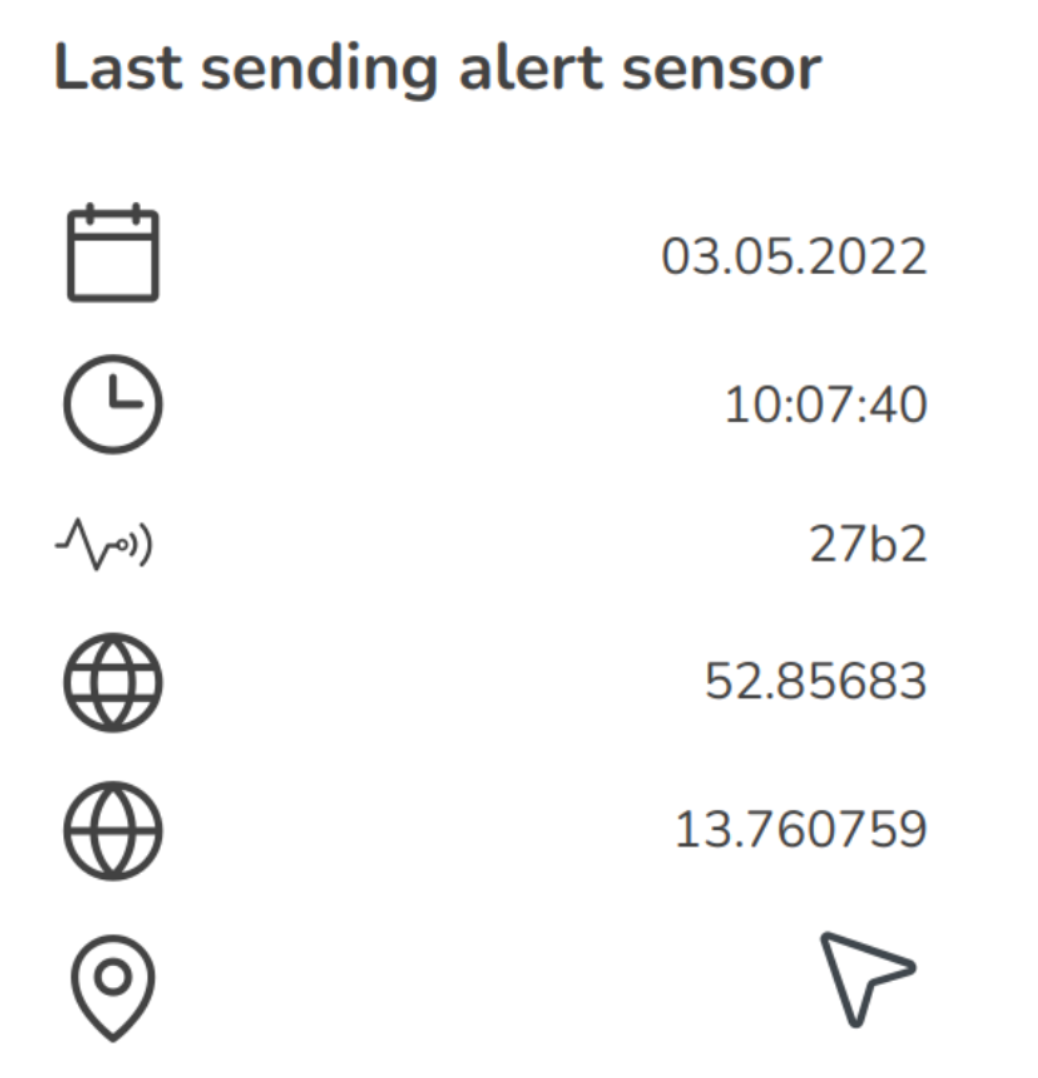
\includegraphics[width=4cm]{app_label_icon}
  \caption{Darstellung mit Icons als einzigem Label}
  \label{fig:app_label_icon}
\end{figure}

Doch es ist einfach, Rückfragen oder Fehlinterpretationen seitens des Nutzers zu vermeiden, indem man einfach eine Textbeschriftung neben dem Symbol hinzufügt.

\begin{figure}[H]
  \centering
  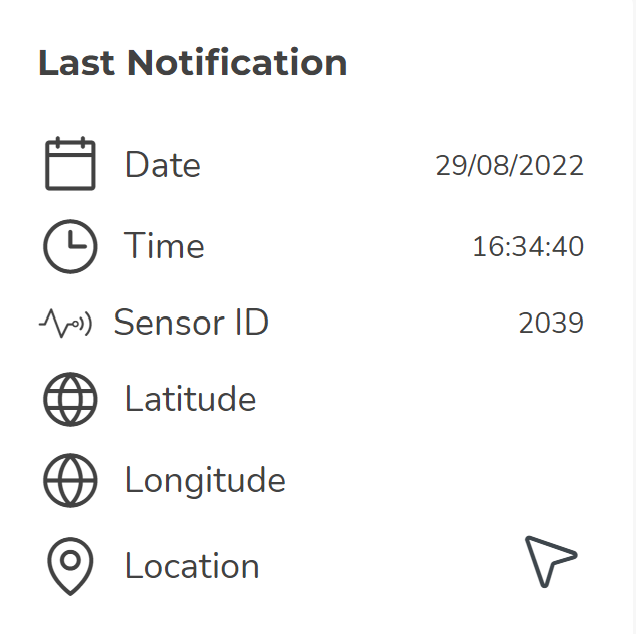
\includegraphics[width=4cm]{app_label_icon_good}
  \caption{Hinzufügen von Textlabels zusätzlich zu den Icons, um die Verwechslung von \ref{fig:app_label_icon} einzuschränken}
\end{figure}


Ein weiteres Unterkriterium betrifft die ortsbezogene Gruppierung der Komponenten einer Schnittstelle nach ihrer Zugehörigkeit und Hierarchie.
In der Tat wird der Benutzer \textit{die verschiedenen Elemente leichter erkennen, wenn sie in einer geordneten Weise präsentiert werden}\cite{bastienscapin}.
Dies hat den Vorteil, dass die Items einer Schnittstelle schneller erlernt und leichter behalten werden können.
Die Silvanet-Webschnittstelle ist voll von Stellen, an denen die Hierarchie der Komponenten betont werden könnte.
Ein gutes Beispiel ist das folgende Filtermenü:

\begin{figure}[H]
  \centering
  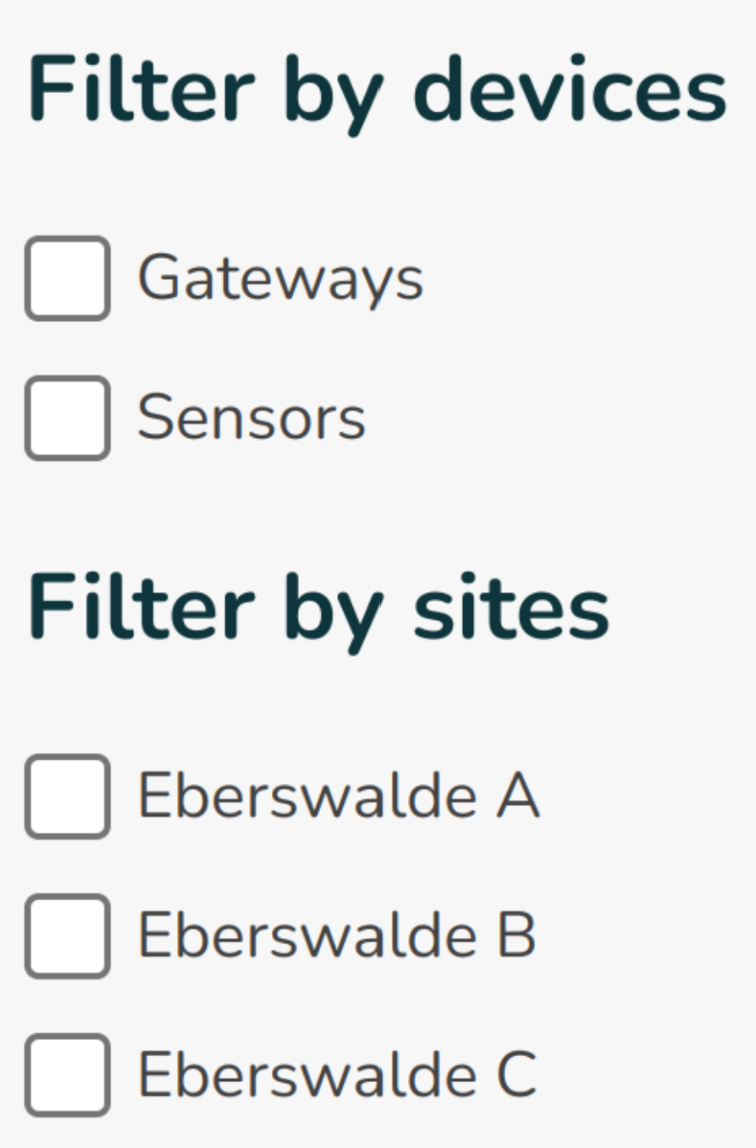
\includegraphics[width=4cm]{app_filter_menu_bad}
  \caption{Menü mit geringer hierarchischer Unterscheidung}
  \label{fig:app_filter_menu_bad}
\end{figure}

Doch schon das Hinzufügen von etwas mehr Padding auf der Ebene der Items hilft dem menschlichen Auge, eine Hierarchie zu visualisieren, in der die Items zu dem Titel über ihnen gehören.
Darüber hinaus kann ein Kollaps-System verwendet werden, um die Zugehörigkeit zu einer Kategorie weiter zu spezifizieren.
Dieses System kann einfach durch ein Chevron-Symbol verdeutlicht werden.

\begin{figure}[H]
  \centering
  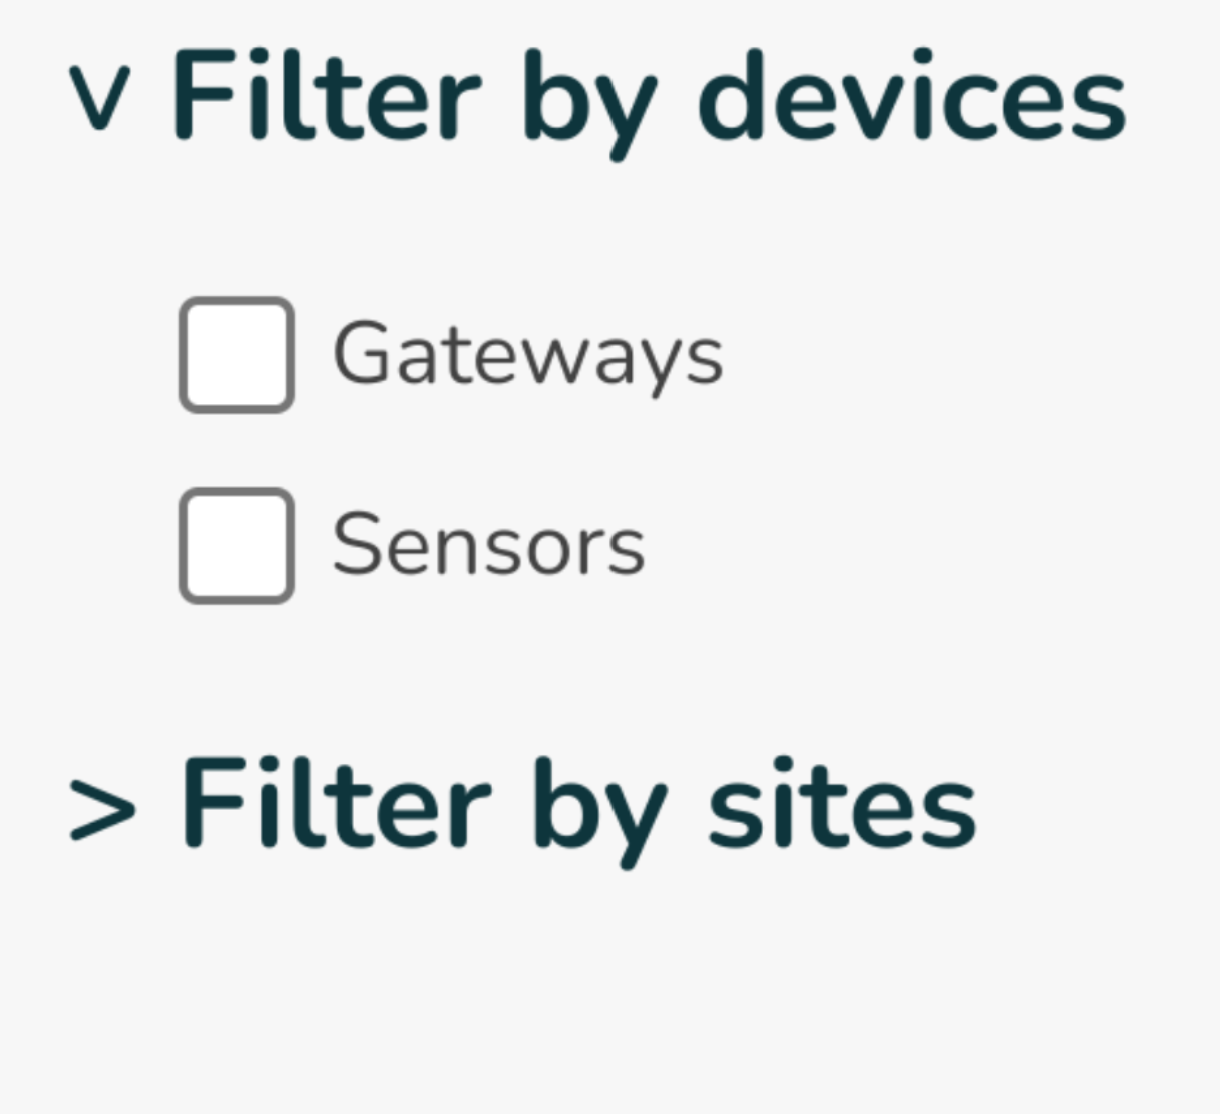
\includegraphics[width=4cm]{app_filter_menu_good}
  \caption{Neustrukturierung des Menüs \ref{fig:app_filter_menu_bad}, um die Sichtbarkeit der Hierarchie zu erhöhen}
\end{figure}

Ähnlich wie das Unterkriterium Unterscheidung nach Ort gibt es auch das Unterkriterium Unterscheidung nach Formatierung.
Ein gutes Beispiel dafür, wie dieses Kriterium angewendet werden könnte, ist die Anzeige von Namen und Kennungen von Einheiten wie Sensoren oder Gateways.
In der folgenden Abbildung sehen wir eine Liste von Geräten, die mit einem Namen identifiziert werden, der eine Art Identifikator enthält.
Da die Kennung eines Geräts nur als Text angezeigt wird, ist die Identifizierung langsamer.
In dieser Form ahnt der Nutzer nicht, dass es möglich ist, mit diesem Text zu interagieren, indem er ihn anklickt.
Dies ist jedoch der Fall, da es möglich ist, auf die Detailseite eines Geräts zu navigieren, indem man auf diese Art von Kennung klickt.

\begin{figure}[H]
  \centering
  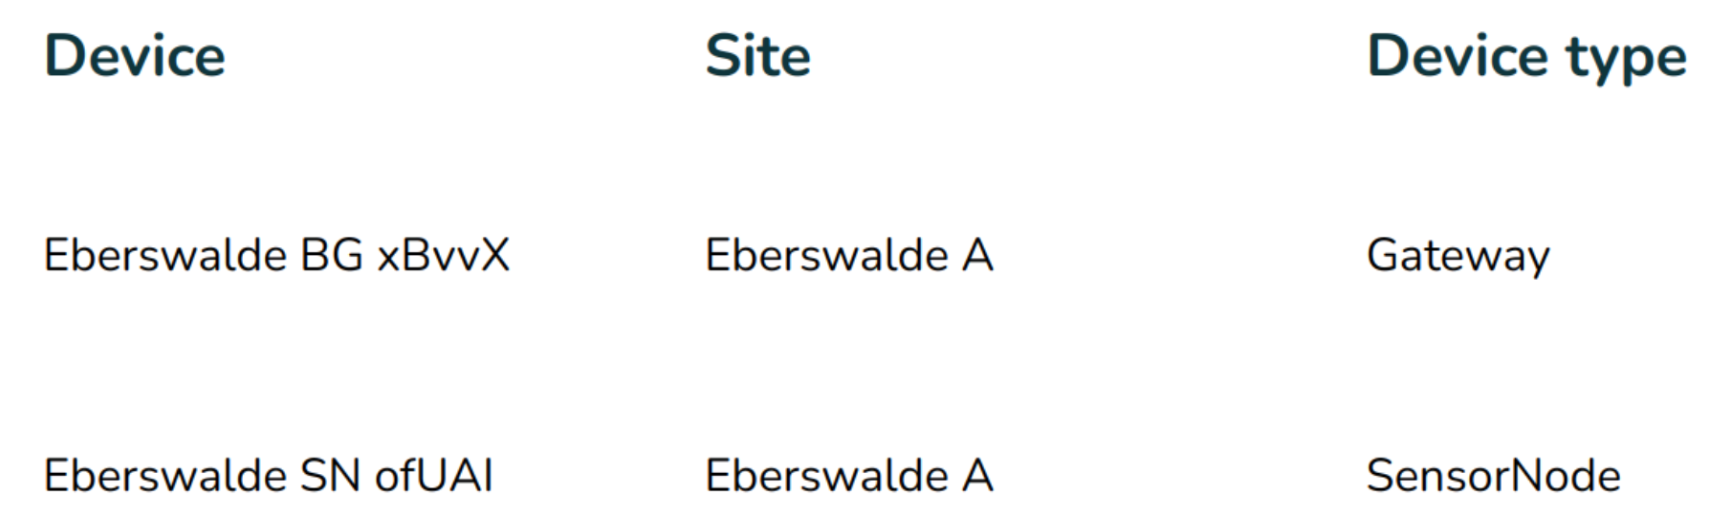
\includegraphics[width=7cm]{app_format_devices_id_bad}
  \caption{Anzeige von Geräteentitäten ohne Differenzierung der Formatierung}
  \label{fig:app_format_devices_id_bad}
\end{figure}

Das Hinzufügen eines einfachen/reinen Designs eines Tags oder einer Schaltfläche (Hintergrund mit schlichter Farbe und einem abgerundeten, ausgeprägten Rand) zu den Gerätekennungen je nach Gerätetyp hilft den Nutzern, eine dichte Benutzeroberfläche schneller zu lesen.

\begin{figure}[H]
  \centering
  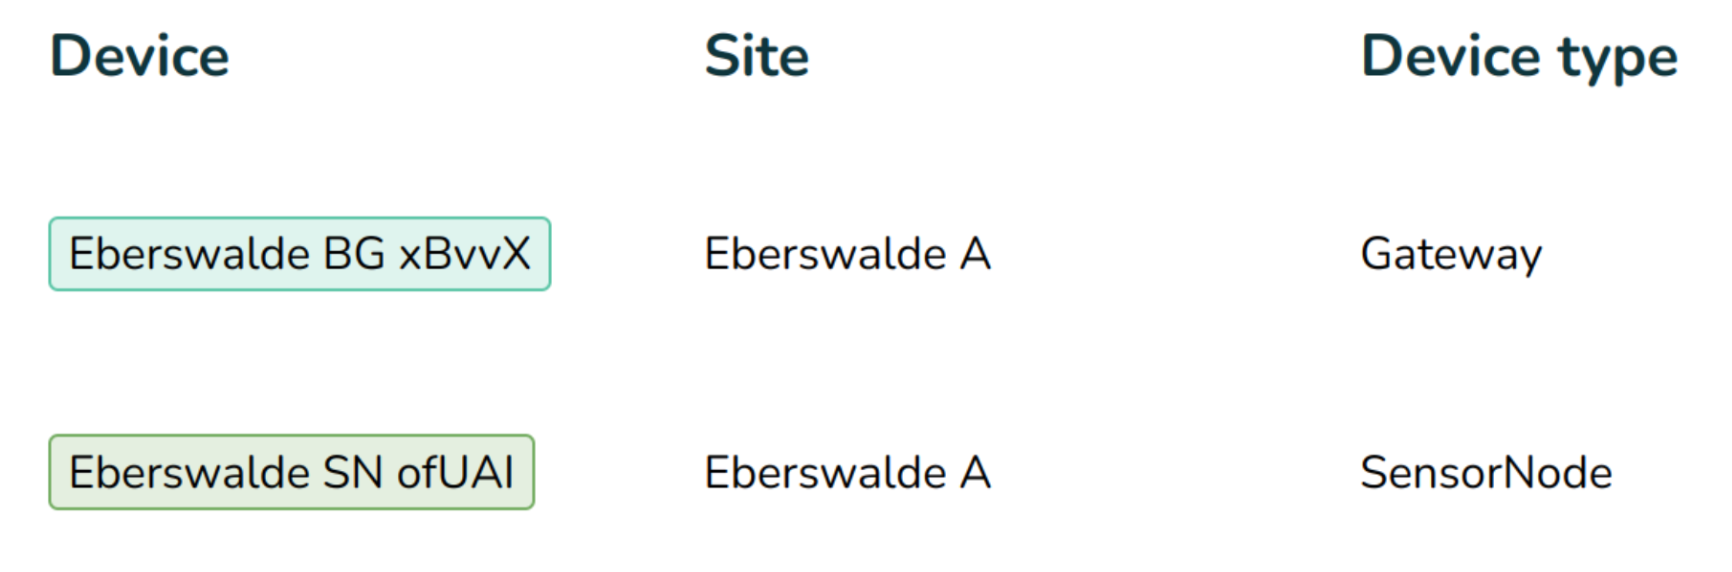
\includegraphics[width=7cm]{app_format_devices_id_good}
  \caption{Anzeige von Geräteentitäten mit Differenzierung der Formatierung}
  \label{fig:app_format_devices_id_good}
\end{figure}

Dies erleichtert dem Benutzer das Erlernen der Fähigkeit, diese Art von Entitäten über die gesamte Schnittstelle zu erkennen.

\begin{figure}[H]
  \centering
  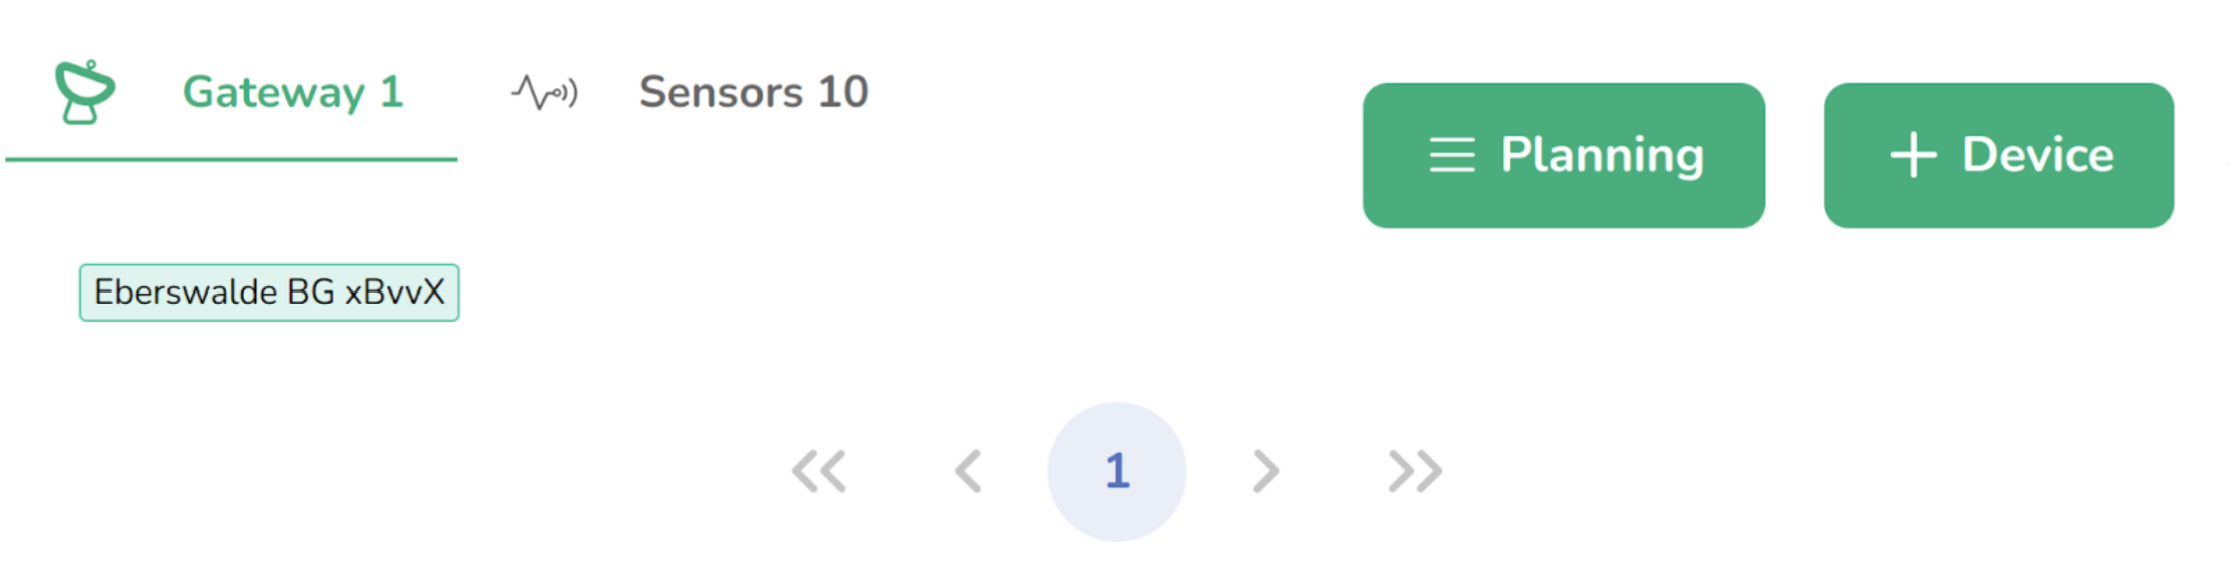
\includegraphics[width=9cm]{app_format_devices_id_extended}
  \caption{Gemeinsame Nutzung der Formatierung der Entität Gerät}
  \label{fig:app_format_devices_id_extended}
\end{figure}

Eine der Säulen der Benutzerführung zur Aufgabenerledigung ist das \textit{sofortige Feedback} nach einer Aktion.
In allen Fällen sollte eine schnelle Antwort des Schnittstelle mit Informationen über die angeforderte Transaktion und ihr Ergebnis erfolgen.
Leider verarbeitet die Silvanet-Anwendung nur sehr wenig Feedback zu den Aktionen des Benutzers.
Aufgrund der geringen Effektivität und des Zeitmangels bei der Entwicklung der Schnittstelle wird dem Nutzer nur ein kleiner Teil der Erfolge gezeigt.
Bei den meisten Knöpfen, die angeklickt werden, erhält der Nutzer z. B. kein Feedback. In den meisten Fällen wird die Aktion relativ schnell ausgeführt und der Nutzer schließt daraus auf einen Erfolg.
Es kann jedoch vorkommen, dass die Aktion einige Zeit in Anspruch nimmt (z. B. bei einer schlechten Verbindung), und der Nutzer sollte darüber informiert werden, dass die Anfrage bearbeitet wird.

Es ist daher von entscheidender Bedeutung, dass eine angeklickte Schaltfläche, die eine Aktion ausführt, dem Benutzer eine Schnittstelle präsentiert, die den Ladevorgang veranschaulicht.
Dies kann leicht durch die Verwendung einer \ac{UI}-Komponente namens Spinner erreicht werden.

\begin{figure}[H]
  \centering
  
\includegraphics[width=5cm]{app_example_loader}
  \caption{Beispiel einer Schaltfläche, die nach dem Anklicken einen Spinner darstellt, der eine laufende Aktion anzeigt}
  \label{fig:app_example_loader}
\end{figure}

Ein ähnliches Problem ist bei der Anzeige von Sensoren auf der interaktiven Karte zu erkennen.
Tatsächlich werden die verschiedenen Geräte an einem Standort im Hintergrund abgerufen, sobald der Nutzer auf eine bestimmte Ebene zoomt.
Wenn die Internetverbindung jedoch nicht schnell genug ist oder der Benutzer schnell zoomt, hat der Benutzer nicht das Gefühl, dass im Hintergrund eine Abfrage stattfindet, da nichts passiert, und sucht daher vergeblich nach Sensoren auf der Karte.

\begin{figure}[H]
  \centering
  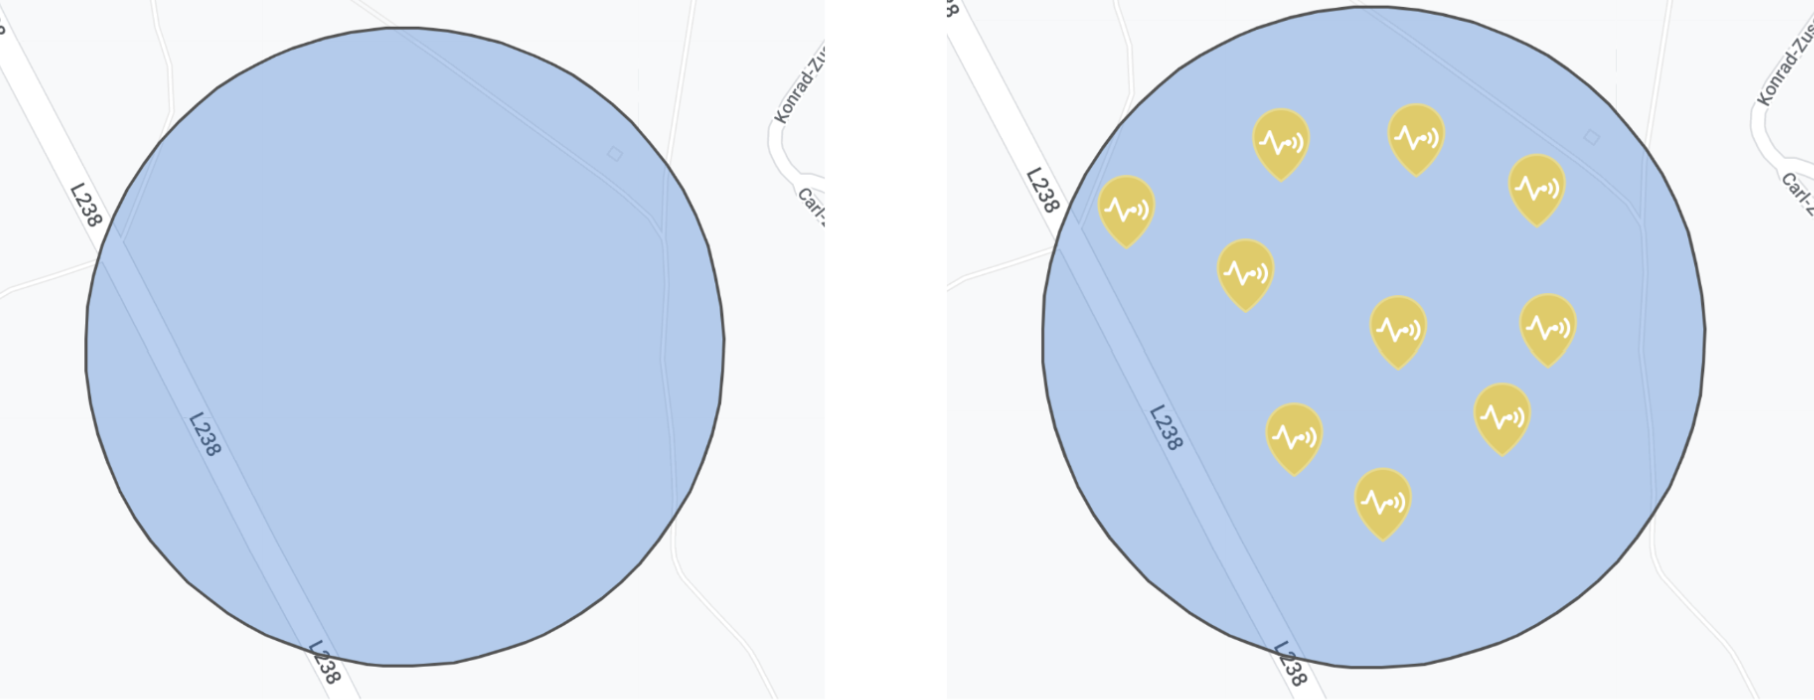
\includegraphics[width=9cm]{app_sensors_map_loading}
  \caption{Bei einer langsamen WLAN-Verbindung zoomt der Benutzer in eine \textit{Site} (blauer Bereich), aber es scheint nichts zu passieren. Erst nach einigen Sekunden sind die Sensoren sichtbar.}
  \label{fig:app_sensors_map_loading}
\end{figure}

Dasselbe Problem findet sich in der überwiegenden Mehrheit der Schnittstelle, wo die meisten Abfragen (fetch/\ac{XHR}) dem Benutzer nicht angezeigt werden.
Sehr oft kann man mit einer langsamen Verbindung auf einen Bereich der Schnittstelle zugreifen, der leer ist, weil die Daten gerade geetcht werden.
Es gibt jedoch viele \ac{UI}-Komponenten, die einem Benutzer mitteilen, dass eine Aktion im Hintergrund abläuft.
Eine der am besten geeigneten Komponenten für diese Art von Feedback ist das Skeleton, das einerseits den Benutzer über das Laden einer Seite oder eines Teils einer Seite benachrichtigt, andererseits aber auch die wahrgenommene Wartezeit des Benutzers verkürzt.
Die Studie von Bill Chung in seinem \textit{Artikel Everything you need to know about skeleton screens}\cite{skeletonScreens} zeigt, dass Skeleton-Komponenten am besten gegen einen einfachen Spinner oder eine leere Seite abschneiden, was die Reduzierung der Wartezeitwahrnehmung betrifft.

Das in der Silvanet-Schnittstelle verwendete Library, PrimeNg, bietet eine Skeleton-Komponente out of the box und wird eine einfache Implementierungslösung für dieses Issue ermöglichen.

\begin{figure}[H]
  \centering
  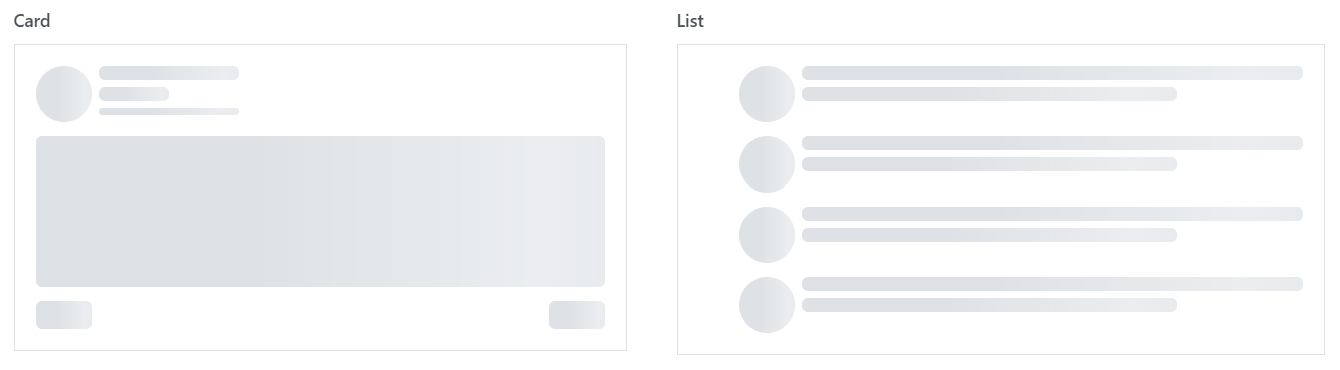
\includegraphics[width=\textwidth]{primeng_skeletons}
  \caption{Beispiel für \ac{UI}-Komponenten-Skeletons, die vom Library PrimeNg bereitgestellt werden}
  \label{fig:primeng_skeletons}
\end{figure}

\subsection{Workload} \label{sec:workload}

Das Unterkriterium \textit{Brevity / Concision} besagt, dass eine Schnittstelle den wahrnehmungsbezogenen und kognitiven Aufwand für einzelne Eingaben oder Ausgaben begrenzen sollte, da die kurzfristige Erinnerungsfähigkeit eines Nutzers begrenzt ist.
Leider erfüllt die Silvanet-Anwendung dieses Kriterium nicht, wenn es darum geht, dem Benutzer metrische Daten anzuzeigen.
Die Anwendung erfordert, dass Flächen mehrfach angezeigt werden, sei es die Fläche einer Site oder die sensorische Abdeckung eines Sensors.
Wenn jedoch keine Skalierung der Daten vorgenommen wird, wird es für einen Nutzer sehr schnell schwierig, diese Daten zu bewerten, wie man im nächsten Screenshot sehen kann:

\begin{figure}[H]
  \centering
  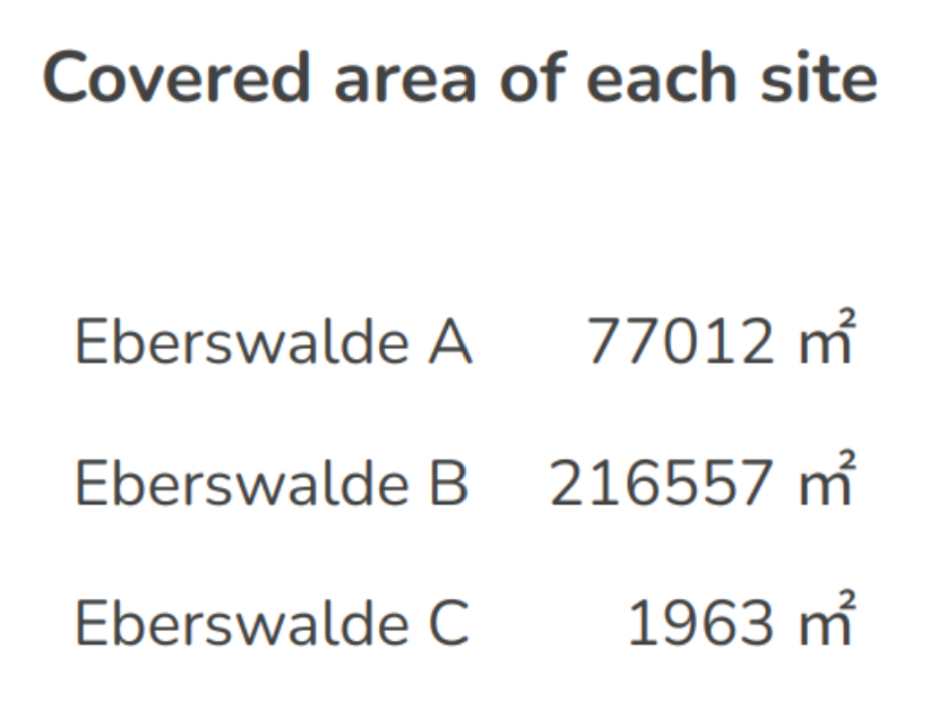
\includegraphics[width=5cm]{app_area_mesure_bad}
  \caption{Messung von nicht skalierten Bereichen, die die kognitive Belastung der Schnittstelle verstärken}
  \label{fig:app_area_mesure_bad}
\end{figure}

Das Unterkriterium \textit{Brevity / Minimal} Actions weist auf ein allgemeines Problem der Silvanet-Anwendung hin, nämlich den Mangel an eindeutigen URL-Zugriffen auf einen Teil der Anwendung.
Die Anwendung erfolgt hauptsächlich durch das Öffnen und Schließen von Popups mittels Knopfdruck.
In vielen Szenarien muss der Nutzer daher mehrere Klicks ausführen, um zum Stadion zurückzukehren, z. B. vor einer Seitenaktualisierung.
Mit diesem Mangel lässt die Anwendung dem Nutzer nicht viel Freiheit, einfach einen bestimmten Teil der Anwendung zu teilen.

\begin{figure}[H]
  \centering
  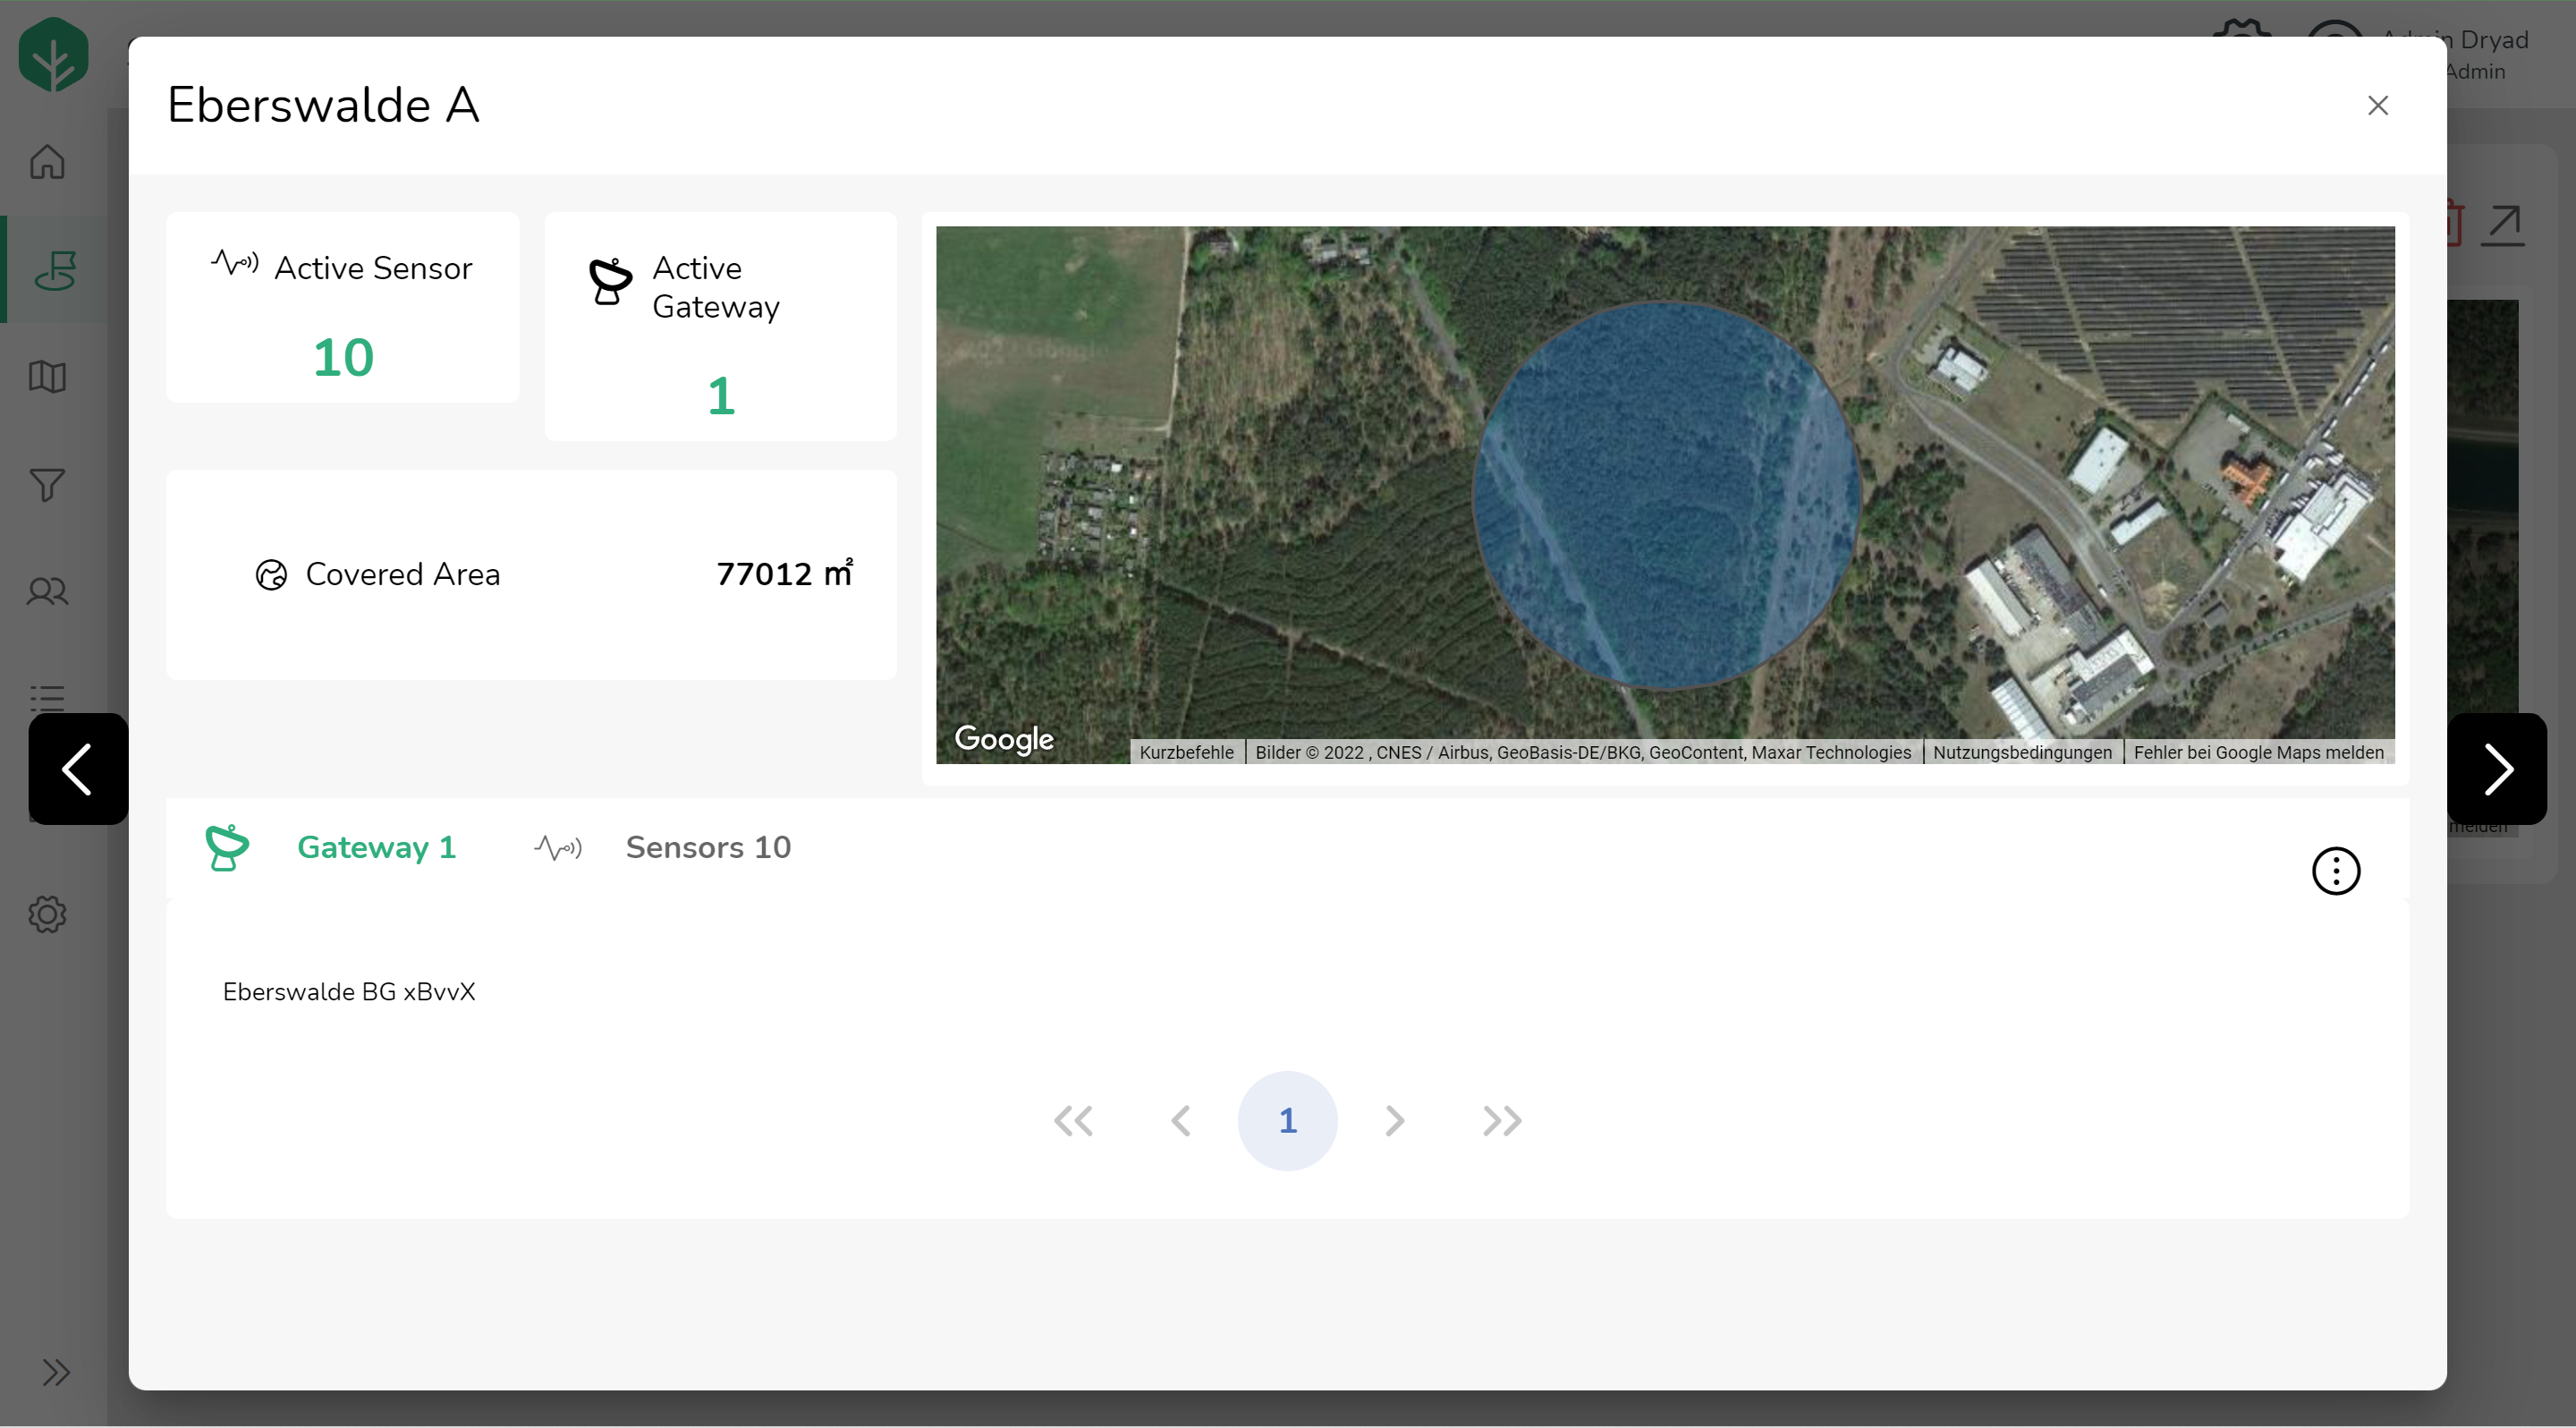
\includegraphics[width=\textwidth]{app_site_details_popup}
  \caption{Popup, das die Details einer \textit{Site} präsentiert}
  \label{fig:app_site_details_popup}
\end{figure}

Eines der markantesten Beispiele ist die Seite mit den Details einer \textit{Site}, die in einem Popup geöffnet wird.
Ein Nutzer kann diese Details nicht direkt mit einem anderen Nutzer teilen, da es keinen Link zum Öffnen des Popups gibt.


\subsection{Explicit Control}

Einer der wichtigsten Aspekte der Silvanet-Anwendung, wenn es um das Kriterium \textit{Explicit Control} geht, sind die Aktionen in Popups.
Wenn ein Popup vom Benutzer geschlossen wird und sich darin ein Formular befindet, wird das Formular so gesendet, als ob es vom Benutzer bestätigt worden wäre.
Dies ist in den Augen eines Benutzers sehr verwirrend, denn eine Schnittstelle sollte ``immer einen Benutzer auffordern, eine explizite ENTER-Aktion durchzuführen, um die Verarbeitung eingegebener Daten einzuleiten''\cite{bastienscapin}.

Das Kriterium \textit{User Control} bezieht sich auf die Tatsache, dass die Benutzer immer die Kontrolle über die Systemverarbeitung haben sollten (z. B. Unterbrechen, Abbrechen, Anhalten und Fortsetzen).
Jede mögliche Aktion eines Benutzers sollte antizipiert werden und es sollten entsprechende Optionen zur Verfügung gestellt werden.
Die silvanet-Anwendung hat an vielen Stellen riskante Aktionen, wie z. B. das Löschen einer \textit{Site} oder das Festlegen, dass eine Waldbrandwarnung ein Fehlalarm ist.
Obwohl diese Aktionen bereits durch einen Bestätigungsdialog geschützt sind, könnte es sinnvoll sein, die Fehlerbehandlung zu verstärken, indem man eine \textit{Vorgang abbrechen}-Aktion hinzufügt.
Dies wird dem Benutzer ein Gefühl der Zuversicht vermitteln, wenn er die Schnittstelle manipuliert, da keine Aktion endgültig ist.
Ein gutes Beispiel für diese Art der Rückgabeaktion ist auf der Gmail-Oberfläche mit dieser Komponente namens \textit{Toast} zu sehen, die es dem Nutzer ermöglicht, das Löschen einer E-Mail rückgängig zu machen:

\begin{figure}[H]
  \centering
  
\includegraphics[width=7cm]{gmail_undo_toast}
  \caption{\textit{Toast}nachricht von Gmail, mit der das Löschen einer E-Mail rückgängig gemacht werden kann}
  \label{fig:gmail_undo_toast}
\end{figure}


\subsection{Adaptability}

Nach den Kriterien von Bastien und Scapin muss eine Schnittstelle, um ergonomisch zu sein, eine Anpassungsfähigkeit an den Benutzer bieten.
Dies wird im Kriterium \textit{Flexibility} hervorgehoben, das sich in der Fähigkeit einer Schnittstelle ausdrücken lässt, sich an die Bedürfnisse eines Nutzers anzupassen.
So wäre es relevant, dass die Schnittstelle von Silvanet ein gewisses Maß an Anpassungsmöglichkeiten bietet.
Ein guter Kandidat wäre die Seite, auf der die verschiedenen \textit{Sites} eines Nutzers vorgestellt werden.
Derzeit besteht diese Liste aus Card-Komponenten, die den Namen des \textit{Sites} und eine Ansicht des \textit{Sites} auf einer interaktiven Karte anzeigen.

\begin{figure}[H]
  \centering
  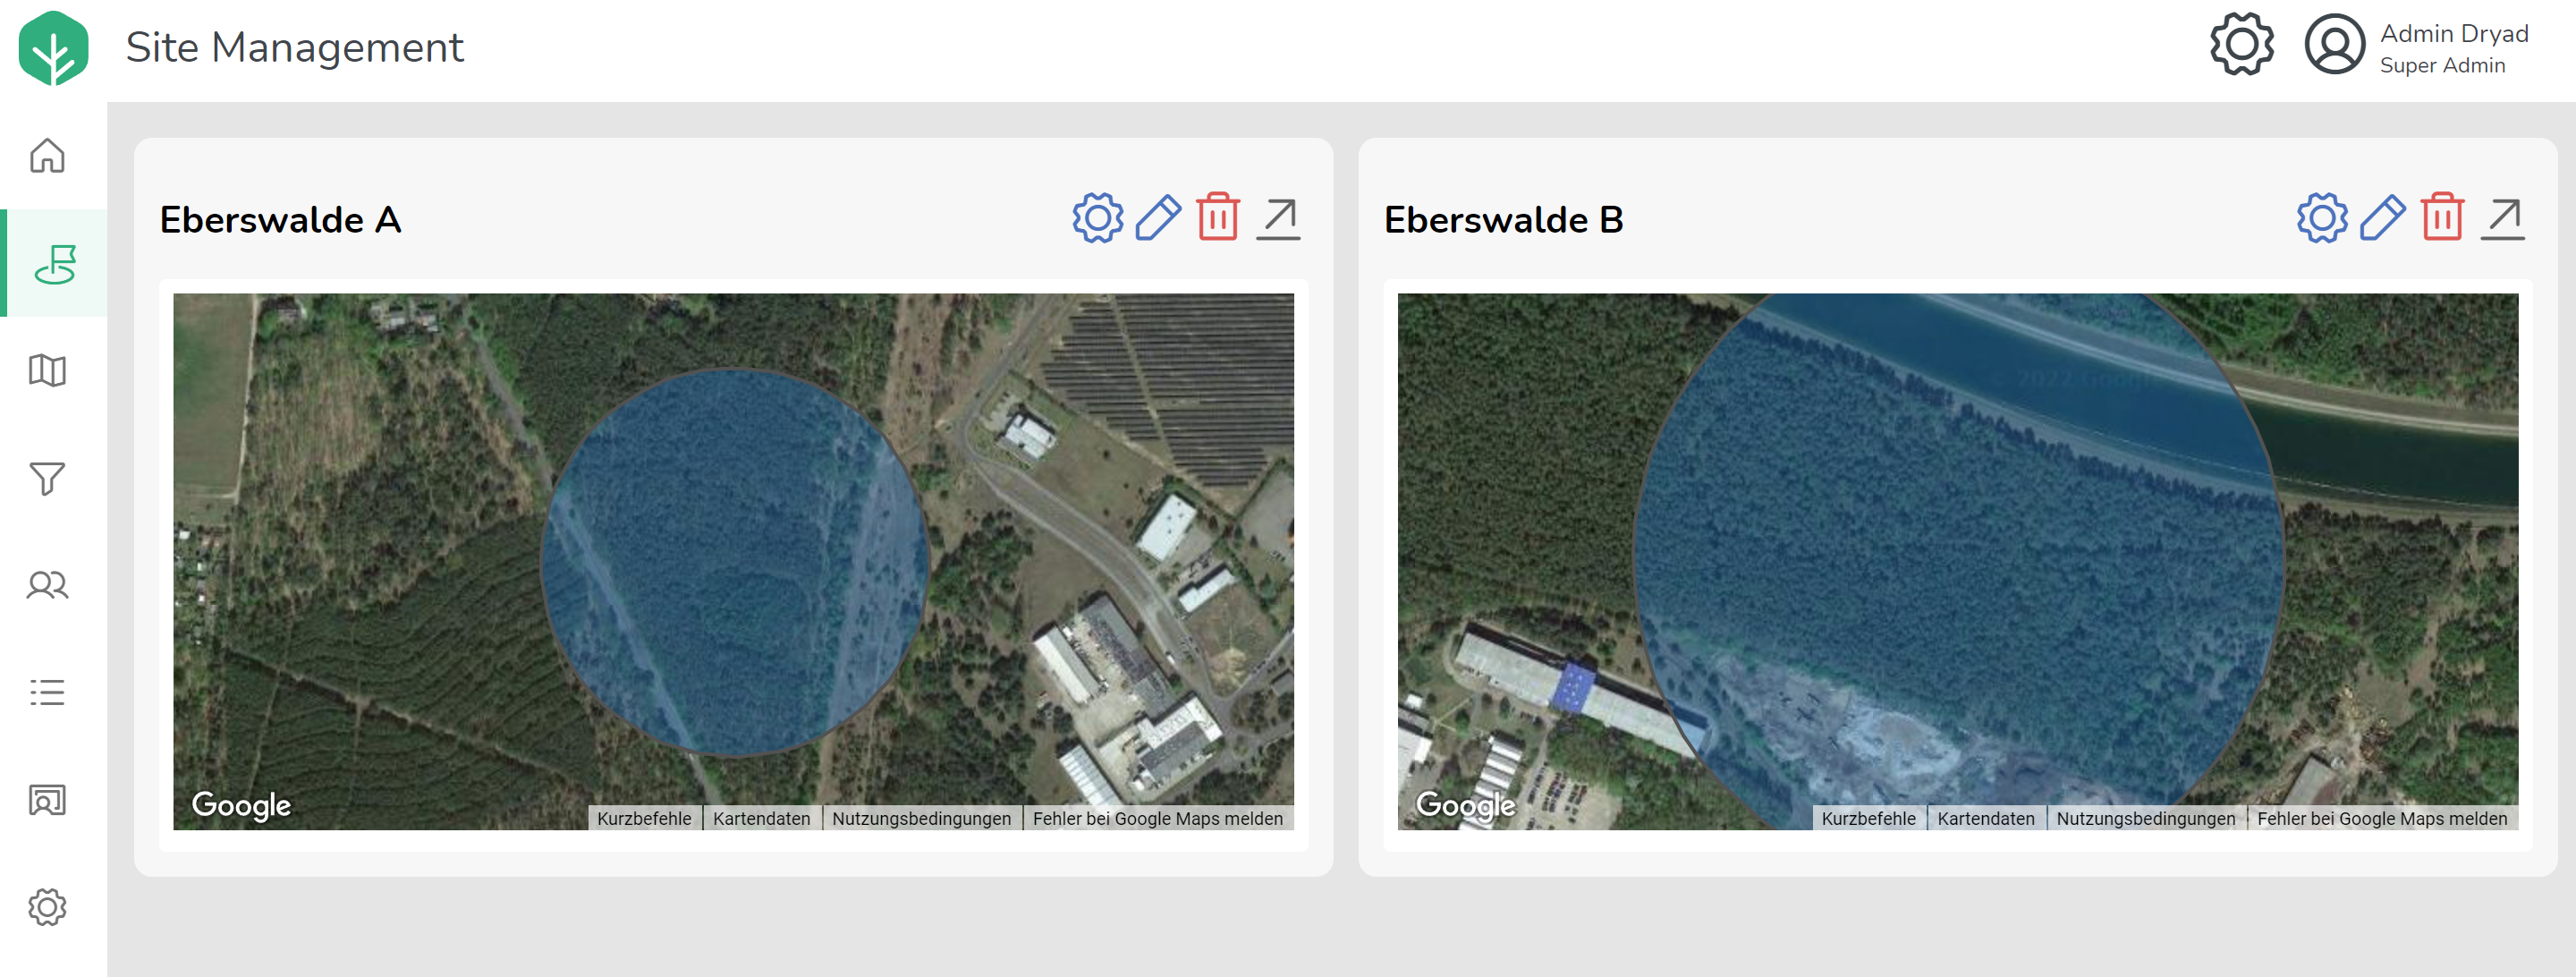
\includegraphics[width=\textwidth]{app_sites_in_sites_list}
  \caption{Seite mit der Liste der \textit{Sites} eines Nutzers}
  \label{fig:app_sites_in_sites_list}
\end{figure}

Auf dieser Seite wäre es möglich, das Auffinden einer bestimmten \textit{Site} in der Liste zu erleichtern, indem man dem Benutzer die Möglichkeit gibt, Änderungen an der \ac{UI} vorzunehmen, um so die Erinnerung an die Schnittstelle zu fördern.
Eine interessante Idee ist es, den Nutzer die Liste nach seinen Vorlieben ordnen zu lassen.
Um das schnelle Erkennen eines Listeneintrags zu erleichtern, könnte es möglich sein, die Hintergrundfarbe der Card-Komponente zu ändern.
Im gleichen Sinne könnte der Nutzer die interaktive Karte durch ein Bild seiner Wahl ersetzen.\\

Ein interessanter Aspekt der Silvanet-Anwendung und ihre Absicht, weltweit nutzbar zu sein.
Dryads Lösung zur Erkennung von Waldbränden sollte allen potenziellen Kunden auf der ganzen Welt angeboten werden.
So muss die Anwendung unabhängig von der Sprache oder der Kultur des Nutzers nutzbar sein.
Aus ergonomischer Sicht ist dies mit einer Vielzahl von Abhängigkeiten verbunden, darunter auch die der \ac{I18n} und der \ac{L10n}.
Die Einführung dieser beiden technischen Verfahren wird als Globalisierung bezeichnet\cite{lisa}.


\subsubsection{\ac{I18n}}

Die Internationalisierung umfasst die Planungs- und Vorbereitungsphasen für ein Produkt, in denen es von vornherein für die Unterstützung globaler Märkte konzipiert wird.
Dieser Prozess bedeutet, dass alle kulturellen Annahmen entfernt werden und alle länder- oder sprachspezifischen Inhalte außerhalb des Produkts gespeichert werden, so dass es leicht angepasst werden kann.
Die Internationalisierung besteht in erster Linie darin, die Funktionalität eines Produkts von einer bestimmten Kultur, Sprache oder einem bestimmten Markt zu abstrahieren, damit die Unterstützung für bestimmte Märkte und Sprachen problemlos integriert werden kann.
In der Welt der Software gibt es viele Beispiele für Designfehler bei der Internationalisierung, wie z. B. nicht übersetzte Texte in Grafiken, nicht übersetzte Screenshots der Anwendung in der Dokumentation oder Telefonnummern, die im Ausland nicht verwendet werden können.

\subsubsection{\ac{L10n}}

Die Lokalisierung bezieht sich auf die tatsächliche Anpassung des Produkts an einen bestimmten Markt.
Sie umfasst die Übersetzung, die Anpassung von Grafiken, die Übernahme lokaler Währungen, die Verwendung korrekter Formulare für Daten, Adressen und Telefonnummern und viele andere Details, einschließlich der physischen Struktur von Produkten in einigen Fällen.
Wenn diese Details in der Internationalisierungsphase nicht vorgesehen waren, müssen sie während der Lokalisierung korrigiert werden, was das Projekt zeitlich und finanziell belastet.\\

Die Globalisierung kann also in einen Kreislauf zwischen \ac{I18n} und \ac{L10n} übersetzt werden, den das Team von Dryad bei der Erstellung ihrer Produkte anwenden könnte.

\begin{figure}[H]
  \centering
  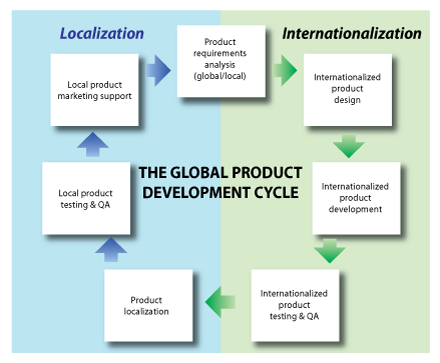
\includegraphics[width=8cm]{globalization_cycle}
  \caption{Darstellung des Globalisierungszyklus eines Produkts}
  \label{fig:globalization_cycle}
\end{figure}


\subsection{Error Management}

Wie in den Empfehlungen zum \textit{Error Management} erwähnt, ist es besser, "Fehler vor der Validierung als danach zu erkennen".
Daher sollte die Schnittstelle erkennen und verhindern Dateneingabefehler, Befehlsfehler oder Aktionen mit zerstörerischen Folgen.
Dies gilt insbesondere für die verschiedenen Formulare von Silvanet, wo die meisten Inputs nicht angeben, welches Format erlaubt ist, und nach dem Absenden des Formulars einen Fehler zurückgeben.
Es soll die Benutzererfahrung verbessern, wenn Sie wissen, dass Sie in dieser Eingabe nur Zahlen eingeben dürfen, dass Leerzeichen verboten sind oder dass Kommazahlen im Format \textit{xx.xxx} geschrieben werden.\\

Es wird daher empfohlen, dass die Fehlermeldungen für den Benutzer klar sind, wenn eine Aktion nicht wie erwartet verläuft.
Die Anwendung, die sich in einem unfertigen Stadium befindet, zeigt immer wieder Fehlermeldungen an, die für den Benutzer irrelevant sind, wie \textit{Error} oder \textit{Ein Fehler ist aufgetreten}.

\begin{figure}[H]
  \centering
  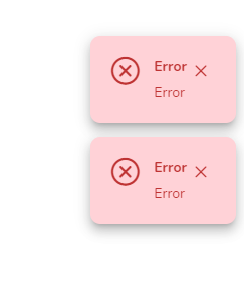
\includegraphics[width=4cm]{app_errors_bad}
  \caption{Screenshot von Push-Benachrichtigungen, die nach einer Fehlbedienung an den Benutzer gesendet werden}
  \label{fig:app_errors_bad}
\end{figure}

Es ist jedoch notwendig, eine ausgezeichnete Qualität der Fehlermeldungen anzubieten, die das Lernen der Nutzer aus den Systemen fördert, indem sie ihnen die Gründe für ihre Fehler und deren Art mitteilen und ihnen beibringen, wie sie ihre Fehler verhindern oder beheben können.

\subsection{Consistency}

Die Kriterien besagen, dass die \ac{UI}-Elemente einer Benutzeroberfläche von Bildschirm zu Bildschirm und von Sitzung zu Sitzung stabil und konsistent sein müssen. Unter diesen Bedingungen ist das Computersystem berechenbarer, das Lernen wird erleichtert und die Anzahl der Fehler wird reduziert.
Ein auffälliges Beispiel für eine solche Inkohärenz findet sich jedoch in einem entscheidenden Element der Anwendung: dem Warnknopf, der bei der Entdeckung eines Waldbrandes angezeigt wird.
Dieser zeigt dem Benutzer den Text "Fire alert", dem das rote Icon eines Sensors vorangestellt ist.
Im gesamten Rest der Anwendung wird ein Feuer jedoch mit dem Icon einer Flamme dargestellt.

\begin{figure}[H]
  \centering
  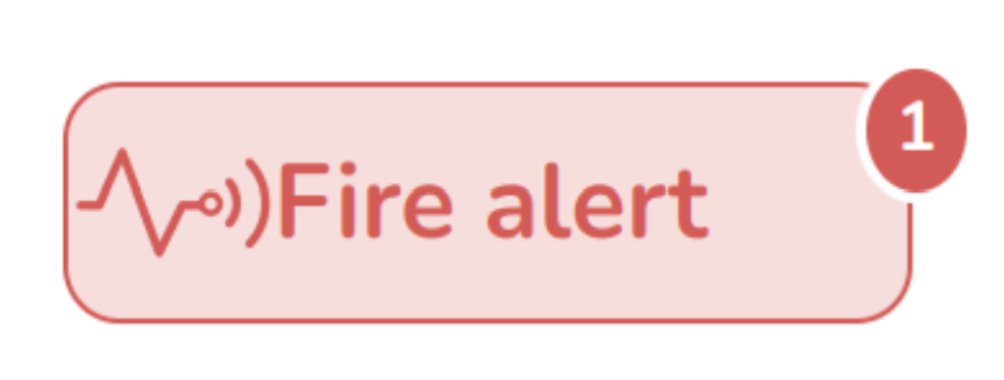
\includegraphics[width=4cm]{app_fire_alert_button}
  \caption{Icon eines Sensors, der auf der Feueralarmtaste verwendet wird}
  \label{fig:app_fire_alert_button}
\end{figure}

\begin{figure}[H]
  \centering
  
\includegraphics[width=2cm]{app_fire_icon}
  \caption{Icon, das in einer Stecknadel verwendet wird, um den Standort eines Feuers auf der Karte anzuzeigen}
  \label{fig:app_fire_icon}
\end{figure}

Damit ein Benutzer einfach einen Zusammenhang zwischen einem Waldbrand und einem Icon herstellen kann, um die Benutzeroberfläche zu entlasten, muss das verwendete Icon für jede Situation einzigartig sein.\\

Im gleichen Sinne hat die Schnittstelle Schwierigkeiten, die Konsistenz bei der Anzeige der Anzahl von Entitäten zu wahren.
Tatsächlich ist das Design des Betrags nicht immer gleich, was dem Nutzer nicht hilft, ihn leicht als Betragswert zu identifizieren.
Ein Beispiel ist die Differenz zwischen dem Betrag für die Geräte und dem Betrag für den Waldbrandalarm.
Eine wird als Abzeichen dargestellt und die andere zeigt einfach den Betrag neben der Entität, die durch einen vertikalen Balken getrennt ist.

\begin{figure}[H]
  \centering
  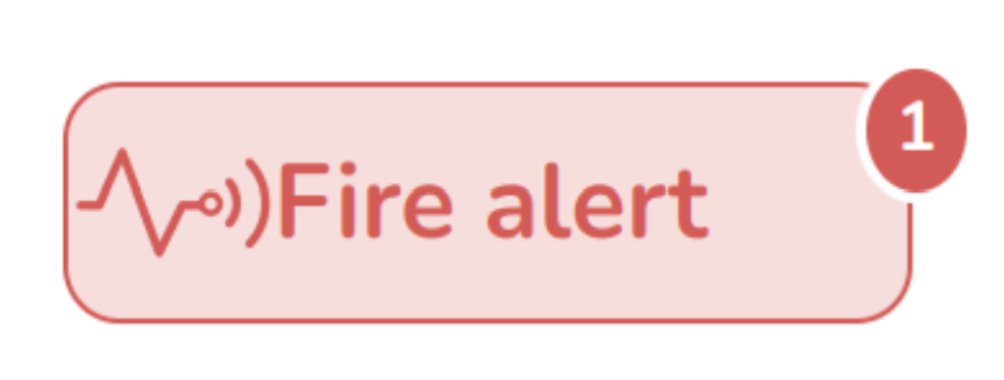
\includegraphics[width=4cm]{app_fire_alert_button}
  \caption{Darstellung eines Betrags als Badge}
  \label{fig:app_fire_alert_button_badge}
\end{figure}

\begin{figure}[H]
  \centering
  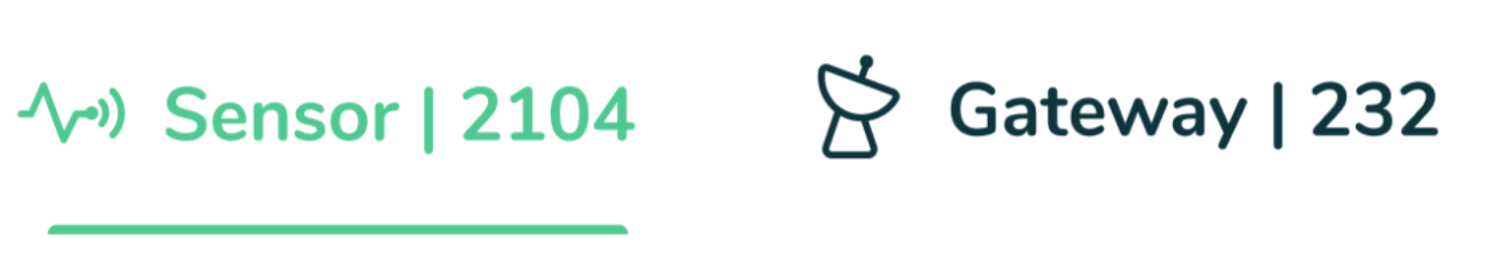
\includegraphics[width=7cm]{app_amount_number}
  \caption{Darstellung eines Betrags als einfache Zahl neben der betreffenden Entität}
  \label{fig:app_amount_number}
\end{figure}

In diesem Fall sollte die \textit{UI} vereinheitlicht werden, indem eine Entscheidung darüber getroffen wird, welche Anzeige bei der Präsentation eines Betrags verwendet werden soll.
Dies wird es dem Benutzer ermöglichen, auf einer komplexen Oberfläche die Beträge einer Entität leicht von anderen Zahlen zu unterscheiden.

\subsection{Zusammenfassung}

Die Analyse der verschiedenen Seiten der Silvanet-Schnittstelle mithilfe der ergonomischen Kriterien von Bastien und Scapin hat bereits viele Mängel aufgedeckt, die die Leistung eines Benutzers beim Verstehen, Lernen und Beherrschen des vorgeschlagenen Systems beeinträchtigen können.
Diese Probleme wurden mithilfe von Tickets im ClickUp-Tool\footnote{\ref{sec:clickup}} in verschiedene Aufgaben aufgeteilt, die unter den verschiedenen Entwicklern aufgeteilt, nach Relevanz und Schwierigkeit der Implementierung priorisiert und schließlich im Scrum-Flow\footnote{\ref{sec:scrum}} verwendet wurden.
Ein Teil der Aufgaben, die sich aus dieser Forschungsarbeit ergeben und die mir zugewiesen wurden, werden im Teil Konzeption\footnote{\ref{chap:konzeption}} der Thesis vorgestellt.
